\section{Electron}
\label{sec:electron}
Electron originally was released as Atom Shell by GitHub at \displaydate{dateAtomShell}~\cite{githubReleaseV010} and downloaded approx. $83\,000\,000$ times\footnote{According to \url{https://npm-stat.com/charts.html?package=electron&from=2013-07-13&to=2022-07-30}}
The intention of the developers was ``to handle the Chromium/Node.js event loop integration and native\\APIs``~\cite{sawicki_2015} for the Atom Editor.
On \displaydate{dateRenameElectron} it was renamed to Electron and announced that the developers want to provide a framework that allows to build desktop applications only with web-technologies.
Many day-to-day apps have been implemented using Electron like Discord, Twitch or even Microsoft Teams.
This has lead to an increasing community which can be expressed numerically based on GitHub Statistics~\cite{GithubElectron} and is shown at Table~\ref{tab:electron:statistics}: \\ \\
\begin{table}[h]
    \begin{tabular} {| c | c | c | c | c |}
        Stars      & Forks     & Watching & Used by    & Contributors \\ \hline
        $130\,000$ & $13\,700$ & $2\,900$ & $244\,568$ & $1\,126$
    \end{tabular}
    \caption{\label{tab:electron:statistics}GitHub Statistics of Electrons Repository}
\end{table}\\ \\
Electron combines both Chromium, an open-source browser and Node.js, an open-source JavaScript-runtime, to provide frontend-based features like rendering \ac{HTML} content as well as \ac{OS}-based features like filesystem access inside one framework.
\subsection{Architecture}
\label{subsec:electron:architecture}
Electrons architecture fundamentally relies on Chromium, which is included in each Electron executable and has a lot common with it.
As Chromium, Electron is based on a multiprocess model, containing of a single process called \textbf{main} and several processes, one for each window, called \textbf{renderer}.
Figure~\ref{fig:electron:model} shows such a multiprocess model structure, where the \texttt{main} process creates and manages multiple \texttt{renderer} processes~\cite{electron-in-action}.
\begin{figure}[ht]
    \centering
    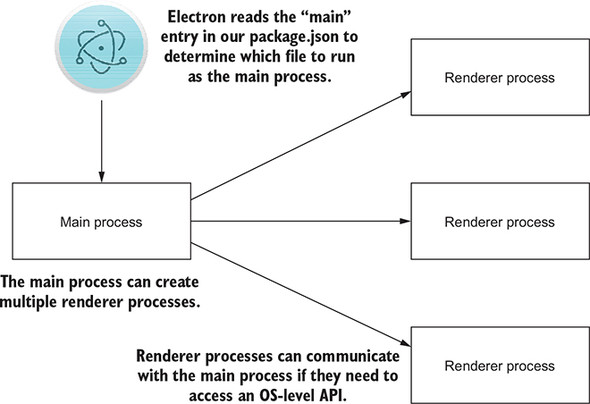
\includegraphics[width=0.4\textwidth]{images/electron-model}
    \caption[Bla]{Multi-process Model Electron from~\cite[Fig. 1.7]{electron-in-action}}
    \label{fig:electron:model}
\end{figure}
\begin{description}
    \item[\textbf{Main}:] \hfill \\ This is the main entry point of the application and responsible for lifecycle management like starting or quitting the app.
    The \texttt{main} process uses so called \texttt{BrowserWindow} module to create and manage each \texttt{renderer} process which is loading web pages into it.
    Since only the \texttt{main} process is running inside a Node.js environment, it is the sole part of the application that can import Node.js modules using \texttt{require}.
    This forces each \texttt{renderer} process to communicate with the \texttt{main} process, if they want to consume system \ac{API}s for purposes like saving files or opening dialogs.
    This communication is called \ac{IPC} and Electrons implementation of it will be discussed in detail at Chapter~\ref{subsubsec:electron:ipc}~\cite{ElectronDoc,electron-in-action}.

    \newpage
    \item[\textbf{Renderer}:] \hfill \\ A \texttt{renderer} process is responsible for rendering web content by loading web pages into it and presenting them to the user at the browser window.
    Additionally, JavaScript code can be loaded and executed inside a \texttt{renderer} process.
    Each \texttt{renderer} process can be created or destroyed by the main process using the \texttt{BrowserWindow} module as mentioned before.
    This leads to the fact, that \texttt{renderer} processes are isolated from each other following the Chromium principles of a multiprocess model and is reasoned by limited affection of
    faulty or malicious code on the entire app.
    The \texttt{renderer} processes are only able to communicate between each other indirectly via the \texttt{main} process or by using \texttt{MessagePorts}.
    ~\cite{ElectronDoc,electron-in-action}.
\end{description}

\subsubsection{Inter Process Communication}
\label{subsubsec:electron:ipc}
As already mentioned the \texttt{main} and \texttt{renderer} processes are only able to communicate using \ac{IPC}.
\begin{figure}[ht]
    \centering
    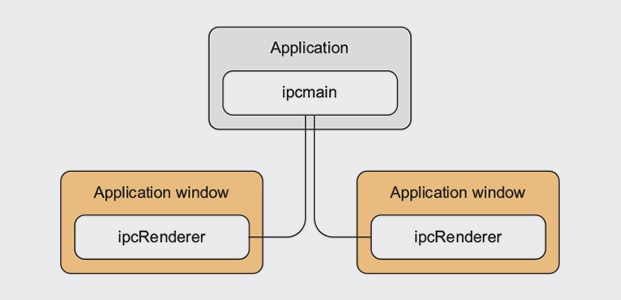
\includegraphics[width=0.4\textwidth]{images/ipcElectron}
    \caption[Bla]{IPC Communication of Electron~\cite[Fig. 6.5]{electron-nwjs}}
    \label{fig:electron:ipc}
\end{figure}
Therefore, Electron provides two modules, one for the \texttt{main} process, called \texttt{ipcMain} and one for \texttt{renderer} process, called \texttt{ipcRender}.
\figref{fig:electron:ipc} points out the process of exchanging data between two or more processes.
Both of them are Node.js \texttt{eventEmitter} modules and capable of executing asynchronously and synchronously communication either uni- or bidirectional.
It should be noticed, that this kind of \ac{IPC} communication is only for \texttt{renderer} to \texttt{main} and vice versa, which can be seen in \figref{fig:electron:ipc}.
A communication between different \texttt{renderer} processes can be archived either indirectly using the \texttt{main} process or directly with \texttt{MessagePorts}.
The advantage of using the direct variant is, that the workload of the \texttt{main} process can be reduced by using a new, hidden \texttt{renderer} process, which serves as a worker for the web content \texttt{renderer}.
A \texttt{MessagePort} can be seen as a communication channel between two \texttt{renderer} processes.
It is once defined inside the \texttt{main} process which informs the \texttt{renderer} processes about belonging \texttt{MessagePorts} from other processes and establishes the connection.
After that, the actual communication does not rely on the \texttt{main} process anymore.
This will reduce workload for the \texttt{main} process in case of message forwarding as well as outsourcing heavy workloads to worker processes~\cite{ElectronDoc}.
\subsubsection{Context Isolation}
Electrons multiprocess model also intends distinct purposes for each process.
As described before only the \texttt{main} process has access to node modules.
In contrast to that only the \texttt{renderer} process has access to \ac{HTML} \ac{DOM}s.
Since using just \ac{IPC} represents a major security issue, Electron introduced a feature called \textbf{Context Isolation}.
This splits the logic of a \texttt{renderer} process into two different contexts.
On the one hand the \texttt{renderer} process as already described and on the other a so called \texttt{preload script}.
The \texttt{preload script} is attached to the \texttt{main} process at the creation of the \texttt{BrowserWindow} module.
It has access to both node modules and \ac{HTML} \ac{DOM}s at its own context and will be executed before the \texttt{renderer} process loads the web page into it.
Although the \texttt{preload script} and the \texttt{renderer} process do both own a window object, which provides the displayed browser window, it is not the same object since they are both running at
different contexts.
The \texttt{preload script} consists of a \texttt{contextBridge} module which is responsible for safely exposing selected properties of the \texttt{main} process to the \texttt{renderer} and vice versa.
Inside this module an \ac{API} can be defined for providing access with \ac{IPC} objects to resources of different processes~\cite{ElectronDoc}.

\subsection{Frontend}
\label{subsec:electron:frontend}
The frontend part of an Electron-based application consists of the Chromium content module and provides all the core features that are required to render \ac{HTML} content
or access web-\ac{API}s.
It is important to notice, that the content module is not equal to the Chrome web-browser since the web-browser wraps around the content module, but provides
several features, the content module does not provide, like managing bookmarks, spellchecking, safe-browsing or securely saving passwords.
The content module itself includes two parts.
A browser engine called \textbf{Blink} and a JavaScript engine called \textbf{V8}~\cite{electron-in-action}.
\begin{description}
    \item[\textbf{Blink}:] \hfill \\ Blink serves as a browser engine inside the Chromium content module and therefore is responsible for translating \ac{HTML} documents to the actual view, a user gets presented.
    Originally Chromium used Webkit as browser engine, which was developed and maintained by Apple, but fundamental disagreements between Apple with its restrictive policy and Google led to the fact,
    that Google forked the Webkit engine and uses it as a grounding for their own engine~\cite{heiseBlink}.
    It relies on the same architecture as mentioned at Chapter~\ref{subsec:electron:architecture}, whereas Blink is running inside a \texttt{renderer} process and uses one main thread
    and multiple worker threads that do the layout calculations~\cite{blinkGoogle}.
    \item [\textbf{V8}:] \hfill \\ V8 is written in C++ and responsible for compiling and executing JavaScript code as well as memory management like allocation or garbage collection.
    It can be seen as the executing background part of the content module, which transforms JavaScript code into C++ code, which in turn is translated into machine-readable byte-code,
    but it also provides the possibilities for developers to write own C++ applications that can expose their functions to JavaScript code to add new features or improve performance of execution~\cite{V8Doc}.

\end{description}
Summarized the content module provides all features to Electron that are necessary to develop a classical browser application.
But since classical browser applications are restricted by the \ac{OS} for example in case of filesystem access, the use-cases are limited.
This is the reason, Electron has combined the content module with the Node.js runtime.
%each view is rendered at a separate process, called \textbf{renderer}.
%The reason for this is that faulty or malicious code is limited in its affection at the whole app.
%Each process is controlled by a single process, which is also the entry point of the app, called \textbf{main}.

\subsubsection{Backend}
\label{subsec:electron:backend}
As backend for all Electron-based applications the Node.js runtime is used.
Node.js is a framework allowing developers to implement server-side applications using JavaScript, and as the Chromium content module of Chapter~\ref{subsec:electron:frontend} it utilizes V8 to execute JavaScript code, but also provides more functionalities like the mentioned filesystem access or the possibility of extern module import.
Furthermore, a pack\-age manager, called \ac{NPM}, with ``more than one million packages``\footnote{\url{https://www.npmjs.com/}} is included.
This amount of packages is a result of an increasing popularity Node.js experienced since its release, providing the capabilities to implement a wide-range of applications.
The reason for utilizing Node.js runtime as a backend for all Electron applications is its privileges.
At traditional web-applications, the client-side is restricted through the \ac{OS} to consume or request data from a third party \ac{API}\@.
Because of that, the client has to request the server, which then is consuming the third party \ac{API}\@.
Since Node.js has these privileges, the detour at the server-side falls away, guaranteeing Electron applications these accesses at the client side~\cite{electron-in-action, electron-nwjs}.


